\section{Signed residuals, the exact returned core, and a compact correction}
\label{irc:section}

This section corrects the unsigned target in the earlier continuation.
It then calculates the complete chart transition and the actual affine
state at the selected third return.  That state supplies an explicit
unforced local continuation.  A flat interpolation and a compact
streamfunction correction connect it to the retained finite field,
with every transition and cutoff contribution displayed.  The
construction is finite and local; its force cost is not claimed to
satisfy an infinite-stage budget.

\subsection{The signed force jets and the unsigned-target defect}

Use the three-index notation of Section~\ref{ibc:section}.  In this
subsection only, write $T_\alpha=\partial^\alpha\widetilde\vartheta$,
$V_{i,\alpha}=\partial^\alpha\widetilde v_i$,
$P_\alpha=\partial^\alpha\widetilde\pi$,
$U_{i,\alpha}=\partial^\alpha\mathcal U_i$,
$D_{ki,\alpha}=\partial^\alpha\mathcal D_{ki}$ and
$G_{i,\alpha}=\partial^\alpha\mathcal G_i$.
These are signed functions, with no norm taken.  Let $e_1,e_2,e_t$
denote index shifts, distinct from the physical vector $e_2=(0,1)$.
Repeated differentiation gives the exact signed arrays
\begin{align}
 R^\theta_\alpha={}&T_{\alpha+e_t}
 +\sum_{i=1}^2\sum_{\beta\leq\alpha}\binom\alpha\beta
 \left[(U_{i,\beta}+V_{i,\beta})T_{\alpha-\beta+e_i}
       +V_{i,\beta}G_{i,\alpha-\beta}\right]
 -\delta_*\sum_{i=1}^2T_{\alpha+2e_i},
 \label{irc:signed-scalar}\\
 R^u_{k,\alpha}={}&V_{k,\alpha+e_t}
 +\sum_{i=1}^2\sum_{\beta\leq\alpha}\binom\alpha\beta
 \left[(U_{i,\beta}+V_{i,\beta})V_{k,\alpha-\beta+e_i}
       +D_{ki,\beta}V_{i,\alpha-\beta}\right]\nonumber\\
 &+P_{\alpha+e_k}-\delta_*\sum_{i=1}^2V_{k,\alpha+2e_i}
       -\mathbf1_{k=2}T_\alpha.
 \label{irc:signed-vector}
\end{align}
They equal $\partial^\alpha\widetilde e_\theta$ and
$\partial^\alpha\widetilde e_{u,k}$, respectively, by the product
rule.  Applying the triangle inequality after these equalities gives
\eqref{ibc:scalar-array}--\eqref{ibc:array-bound}.

\begin{proposition}\label{irc:unsigned-defect}
The unsigned majorants are not necessary force bounds.  On the closed
unit ball, the exact fields
\[
 \widetilde\vartheta(y,\tau)=y_2,\qquad
 \widetilde v=0,\qquad \widetilde\pi=y_2^2/2,\qquad
 \mathcal U=\mathcal D=\mathcal G=0
\]
have identically zero scalar and vector residuals for every
$\delta_*>0$, whereas $\mathsf E^u_{2,0}=2$.
Furthermore, on a duration-$L$ cylinder, bounds
$\max_k\mathsf E^u_{k,0}\leq\epsilon$ imply
$\|\widetilde\vartheta\|_\infty\leq\epsilon$ and, for an increment
starting at $\widetilde v(\cdot,0)=0$,
$\|\widetilde v_k(\cdot,L)\|_\infty\leq L\epsilon$.
\end{proposition}

\begin{proof}
Here $\nabla\widetilde\pi=y_2e_2=\widetilde\vartheta e_2$,
$\Delta\widetilde\vartheta=0$, and every velocity term is zero.
The signed residuals therefore vanish.  The unsigned second momentum
row contains $\|\partial_2\widetilde\pi\|_\infty+
\|\widetilde\vartheta\|_\infty=1+1$, with all its other terms zero.
For the second assertion, all summands in $\mathsf E$ are nonnegative.
Its second momentum row contains $\mathsf T_0$, and each momentum row
contains $\|\partial_\tau\widetilde v_k\|_\infty$.  Integration from
zero to $L$ proves the asserted endpoint bound.  Thus requiring these
majorants to tend to zero on uniformly bounded durations excludes
increments with a fixed nonzero temperature or velocity amplitude,
even when their actual force cancels.  The example is local and
noncompact; it is not asserted to be a compact packet.
\end{proof}

Consequently \eqref{ibc:target-array} now refers to the norms of
\eqref{irc:signed-scalar}--\eqref{irc:signed-vector}.  The old
unsigned target is retained only as a sufficient estimate, with its
earlier source version preserved in the main's provenance directory.

\subsection{Exact receiving map for a correction}

Let $\mathcal B=(c_q^2/\rho_q)\theta^{<q}$ and
$\mathcal P=(c_q^2/\rho_q^2)p^{<q}$ in the same chart.  Thus
$\nabla\mathcal B=\mathcal G$ and $\nabla\mathcal U=\mathcal D$.
Set
\[
 \mathcal T=\mathcal B+\widetilde\vartheta,\qquad
 \mathcal V=\mathcal U+\widetilde v.
\]
For a correction $(h,z,\kappa)$ with $\operatorname{div}z=0$, replace
$(\widetilde\vartheta,\widetilde v,\widetilde\pi)$ by
$(\widetilde\vartheta+h,\widetilde v+z,\widetilde\pi+\kappa)$.
Subtraction of the complete equations gives
\begin{align}
 \Delta\widetilde e_\theta={}&
 h_\tau+\mathcal V\cdot\nabla h+z\cdot\nabla\mathcal T
 +z\cdot\nabla h-\delta_*\Delta h,
 \label{irc:correction-scalar}\\
 \Delta\widetilde e_u={}&
 z_\tau+(\mathcal V\cdot\nabla)z+(z\cdot\nabla)\mathcal V
 +(z\cdot\nabla)z+\nabla\kappa-\delta_*\Delta z-he_2.
 \label{irc:correction-vector}
\end{align}
Every jet of the updated residual is obtained by differentiating
these identities and adding it to the old signed jet.  In particular,
the correction equation is an equation for the actual signed
functions, before any majorant is introduced.  These formulas also
prove the compatibility constraints on a proposed entry tuple:
$\mathcal D=\nabla\mathcal U$, $\mathcal G=\nabla\mathcal B$,
$\operatorname{tr}\mathcal D=0$, and
$\partial_1\mathcal G_2=\partial_2\mathcal G_1$.
They follow by direct differentiation of the defined pullbacks;
three independently chosen arrays need not be a realizable tuple.

\subsection{The complete chart transition}

Keep the physical $d>0$ and $\delta_*>0$ fixed.  Let two charts have
radii $\rho,\rho'>0$, clocks $c=(\delta_*/d)\rho^2$ and
$c'=(\delta_*/d)(\rho')^2$, and centres $(x_0,t_0)$ and
$(x'_0,t'_0)$.  Define
\[
 a=\rho'/\rho>0,\qquad
 \xi=(x'_0-x_0)/\rho,\qquad \tau_0=(t'_0-t_0)/c.
\]
Write $(\Theta,U,P)$ for the complete scalar, velocity and pressure
pullbacks in the first chart, including every retained layer and
cutoff.  The second chart is exactly
\begin{equation}\label{irc:full-chart}
 \begin{aligned}
 \Theta'(y,s)&=a^3\Theta(\xi+ay,\tau_0+a^2s),\\
 U'(y,s)&=aU(\xi+ay,\tau_0+a^2s),\\
 P'(y,s)&=a^2P(\xi+ay,\tau_0+a^2s).
 \end{aligned}
\end{equation}
This follows from the ratios $c'^2/\rho'$ to $c^2/\rho$,
$c'/\rho'$ to $c/\rho$, and $c'^2/(\rho')^2$ to $c^2/\rho^2$.
It proves, with every argument retained,
\begin{equation}\label{irc:gradient-chart}
 D'=a^2D(\xi+ay,\tau_0+a^2s),\qquad
 G'=a^4G(\xi+ay,\tau_0+a^2s).
\end{equation}
Space-time jets of $\Theta,U,P$ acquire respectively
$a^{3+|\gamma|+2b}$, $a^{1+|\gamma|+2b}$ and
$a^{2+|\gamma|+2b}$; those of $D,G$ acquire
$a^{2+|\gamma|+2b}$ and $a^{4+|\gamma|+2b}$.
The complete scalar and vector forces acquire
$a^{5+|\gamma|+2b}$ and $a^{3+|\gamma|+2b}$.
The chain rule proves each identity; no periodic argument, support
boundary, pressure contribution or older layer is replaced.
The inverse uses $a^{-1}$, $-\xi/a$, and $-\tau_0/a^2$.

For a centred affine snapshot $U(y)=Dy$, $\Theta(y)=G\cdot y$,
the action becomes $(D,G)\mapsto(a^2D,a^4G)$.

\begin{proposition}\label{irc:orbit-classification}
On the exact state space
$\{(D,G):D\in\mathbb R^{2\times2},\operatorname{tr}D=0,\,
G\in\mathbb R^2\setminus\{0\}\}$, two centred affine snapshots are
related by a positive parabolic dilation precisely when
\begin{equation}\label{irc:complete-invariants}
 \frac{G'}{|G'|}=\frac G{|G|},\qquad
 \frac{D'}{\sqrt{|G'|}}=\frac D{\sqrt{|G|}}.
\end{equation}
The radius ratio is then uniquely
$a=(|G'|/|G|)^{1/4}$.  It is a shrinking dilation precisely when
$|G'|<|G|$.
\end{proposition}

\begin{proof}
The action in \eqref{irc:gradient-chart} preserves both displayed
quantities since $a>0$.  Conversely, their equality and the displayed
choice of $a$ give $G'=a^4G$ and $D'=a^2D$ entry by entry.
This proves the full orbit classification, including the direction
and every matrix entry.  For curl $W=D_{21}-D_{12}$ it also gives the
invariant $W/\sqrt{|G|}$.  Thus selection of a radius from $|G|$
cannot change the remaining state coordinates.
\end{proof}

\subsection{The actual third-return affine state}

At the selected return time $t_R$, retain all original constants and
the determinant coordinates of \eqref{tr:coordinates}.  In the
following display $D_{\rm ph}=h^2+a_{\rm ph}^2$ is the source scalar
$D$; $a_{\rm ph}=\sin s_2$ distinguishes it from a radius ratio.
The other source names $b,x,y,g,R,c=A_0\cos s_*$ and
$C=A_0\sin s_*$ are unchanged.  On a common affine neighbourhood,
the full physical fields are
\begin{equation}\label{irc:return-field}
 \theta=G_R\cdot x,\qquad u=\mathcal A_Rx,\qquad p=0,
\end{equation}
where
\begin{align}
 G_R&=-A_0R_\alpha e_2+
       \sum_{j=1}^3K_j\Theta_j\zeta_j,
 \label{irc:return-G}\\
 \mathcal A_R&=\dot\alpha J+
       \sum_{j=1}^3\frac{\Omega_j}{|\zeta_j|^2}
                 J\zeta_j\otimes\zeta_j.
 \label{irc:return-D}
\end{align}
These are restrictions of the complete periodic-profile and
material-cutoff fields, rather than new definitions of those fields.
Indeed $F(s)=s$ on $|s|<s_0$, $P'(s)=F(s)$, and every material cutoff
equals one in a neighbourhood of the origin.  The sums therefore
give exactly their scalar and streamfunction derivatives there.

The return and hold equations give
$\zeta_3=(0,\sqrt R)$, $\Omega_3=0$,
$\zeta_1=(-y,x)/\sqrt R$, and $\zeta_2=(-b,g)/\sqrt R$.
Since $\dot\zeta_{3,1}=0$ on the hold and
$\dot\zeta_3=-D_{<3}^T\zeta_3$, one has
$(D_{<3})_{21}=0$.  At the endpoint it follows also by substitution
of the displayed angular control in \eqref{tr:hold}.  Tracelessness
and \eqref{trc:diffusive-root-bounds} yield
\begin{equation}\label{irc:triangular-return}
 \mathcal A_R=
 \begin{pmatrix}a_R&-W_R\\0&-a_R\end{pmatrix},\qquad
 a_R=\frac{\Omega_1xy}{R}
       +\frac{\Omega_2bg}{D_{\rm ph}R},\qquad
 W_R=2\dot\alpha+\Omega_1+\Omega_2
       \geq c_W\sigma_2/4>0.
\end{equation}
No strain sign is imposed.  The angular inverse gives
$\alpha=s_*+\arctan(y/x)$ at this endpoint.  Therefore, retaining
the base and all three temperature terms,
\begin{equation}\label{irc:exact-return-temperature}
 \begin{aligned}
 (G_R)_1&=\frac{(E_1+c)y+Cx+bE_2}{\sqrt R}
          =\frac{N_3}{\sqrt R}>0,\\
 (G_R)_2&=-\frac{(E_1+c)x-Cy+gE_2}{\sqrt R}
             +K_3\Theta_3\sqrt R.
 \end{aligned}
\end{equation}
Positivity uses the proved positive component $N_3$, not an
unproved sign for $(G_R)_2$.  The nonzero $G_R$ lies in the state
space of Proposition~\ref{irc:orbit-classification}.  At a physical
radius $\rho$ its chart coefficients are exactly
$c_\rho\mathcal A_R$ and $c_\rho^2G_R$; a further radius ratio
multiplies these by $a^2$ and $a^4$.  This preserves all physical
diffusion and clock factors in \eqref{ibc:clock}.

\subsection{An explicit unforced affine continuation}

Put $a=a_R$, $b_0=-W_R$, $g_1=(G_R)_1>0$ and
$g_2=(G_R)_2$, without resetting their values.  For $s=t-t_R$ set
\begin{align}
 \Phi_k(a,s)&=\int_0^s e^{-ka r}\,dr
 =\begin{cases}(1-e^{-ka s})/(ka),&a\ne0,\\s,&a=0,\end{cases}
 \quad k=1,2,3,\nonumber\\
 \Xi(a,s)&=\int_0^s e^{-2ar}\Phi_1(a,r)\,dr
 =\begin{cases}(\Phi_2(a,s)-\Phi_3(a,s))/a,&a\ne0,\\
 s^2/2,&a=0.\end{cases}
 \label{irc:affine-integrals}
\end{align}
Define the complete coefficients
\begin{equation}\label{irc:affine-solution}
 \begin{aligned}
 g_1(s)&=g_1e^{-as},&
 b(s)&=b_0-g_1\Phi_1(a,s),\\
 g_2(s)&=e^{as}\left[g_2-g_1b_0\Phi_2(a,s)
                              +g_1^2\Xi(a,s)\right],&
 A(s)&=\begin{pmatrix}a&b(s)\\0&-a\end{pmatrix},\\
 G(s)&=(g_1(s),g_2(s)),&
 H(s)&=\begin{pmatrix}-a^2&g_1(s)\\g_1(s)&g_2(s)-a^2\end{pmatrix}.
 \end{aligned}
\end{equation}

\begin{theorem}\label{irc:affine-continuation}
For every physical $d>0$, the fields
$\theta_A(x,t)=G(s)\cdot x$, $u_A(x,t)=A(s)x$ and
$p_A(x,t)=x^TH(s)x/2$ solve the unforced equal-diffusion
Boussinesq equations on $\mathbb R^2\times\mathbb R$.
Their temperature and velocity at $t_R$ agree exactly with
\eqref{irc:return-field} on its affine neighbourhood.
For $s\geq0$,
\[
 (\nabla\theta_A)_1=g_1e^{-as}>0,\qquad
 \operatorname{curl}u_A=W_R+g_1\Phi_1(a,s)>0.
\]
All coefficients are finite at every finite $s$.
\end{theorem}

\begin{proof}
The integral formulas, including their $a=0$ values, are smooth
in $a,s$ by their integral definitions.  Differentiation gives
$g_1'=-ag_1(s)$, $b'=-g_1(s)$, and
$g_2'=-b(s)g_1(s)+ag_2(s)$.  Hence
$G'+A^TG=0$.  Direct multiplication retains the full matrix
$A^2=a^2I$ and gives
$A'+A^2+H-e_2G^T=0$.
These two identities are precisely the scalar and momentum
equations; $\Delta(G\cdot x)=0$, $\Delta(Ax)=0$, and
$\operatorname{div}(Ax)=\operatorname{tr}A=0$.
The pressure is symmetric and supplies its displayed gradient.
At $s=0$, $\Phi_k=\Xi=0$, so the temperature and velocity
coefficients are the original ones.  For $s\geq0$,
$\Phi_1\geq0$, which proves both signs.
Exponential and finite integrals prove finiteness at every finite
$s$.  This solution is noncompact.  Its initial pressure need
not equal the old zero pressure, and the equations need not
match the old time jets; the next construction repairs the join.
\end{proof}

\subsection{A flat join with every transition term retained}

The selected finite return has a smooth holding continuation on
some compact interval $I=[t_R,t_R+\epsilon]$: local existence of
its smooth finite vector field and the interior component bounds
prove this.  Denote its affine coefficients by $A_h,G_h,H_h=0$.
They retain the nonstationary temperature diffusion and all older
responses in \eqref{tr:hold}--\eqref{trc:holding}.
Choose $0<\ell<\epsilon$ and $\beta(t)=\eta((t-t_R)/\ell)$.
Set $\Delta A=A-A_h$, $\Delta G=G-G_h$ and $\Delta H=H-H_h$,
and define
\begin{equation}\label{irc:flat-interpolation}
 A_\beta=A_h+\beta\Delta A,\quad
 G_\beta=G_h+\beta\Delta G,\quad
 H_\beta=H_h+\beta\Delta H.
\end{equation}
Let the old affine residual coefficients be
$r_h^\theta=G_h'+A_h^TG_h$ and
$r_h^u=A_h'+A_h^2+H_h-e_2G_h^T$.
The total interpolated core residual is exactly
\begin{align}
 r_\beta^\theta&=(1-\beta)r_h^\theta
             +\beta'\Delta G
             -\beta(1-\beta)(\Delta A)^T\Delta G,
 \label{irc:transition-scalar}\\
 r_\beta^u&=(1-\beta)r_h^u
             +\beta'\Delta A-\beta(1-\beta)(\Delta A)^2.
 \label{irc:transition-vector}
\end{align}
The scalar force is $r_\beta^\theta\cdot x$ and the vector
force is $r_\beta^ux$.  To verify these identities, expand
$A_\beta^TG_\beta$ and $A_\beta^2$ and compare their
quadratic terms with $(1-\beta)$ times the old expression and
$\beta$ times the new zero residual.  The difference is
$-\beta(1-\beta)$ times the two displayed products.  Derivatives
of the interpolation give exactly the $\beta'$ terms.
The pressure and buoyancy are linear and are both retained.
For $t\leq t_R$ the interpolated fields equal the old ones with
every time jet; for $t\geq t_R+\ell$ they equal the explicit
unforced core with every time jet.  Flatness of $\eta$ proves both
joins, including the pressure join.

\subsection{Compact realization over the actual retained parent}

The affine neighbourhood can be chosen uniformly on $I$.
Indeed all phase and material matrix norms have finite maxima there.
Writing $L_j=\sup_I\|M_j^{-1}\|$ and
$Z_j=\sup_I|\zeta_j|$, one possible positive radius is
\[
 r_c=\min\left(1,\frac{s_0}{2\mu},
       \min_{1\leq j\leq3}\frac{\ell_j}{4L_j},
       \min_{1\leq j\leq3}\frac{s_0}{2K_jZ_j}\right).
\]
The unchanged $\ell_j$ are the original material envelope radii.
On $B_{r_c}$ the base and every activated profile are exactly
affine, and every material cutoff is one.  This proves the needed
neighbourhood directly, without extending a local support estimate
to the full third trial family.

Take $\chi\in C_c^\infty(B_{r_c})$ equal to one on
$B_{r_c/2}$.  With $B=-J\beta\Delta A$ symmetric, put
\begin{equation}\label{irc:compact-correction}
 h=\chi\,\beta\Delta G\cdot x,\qquad
 Q=x^TBx/2,\qquad z=J\nabla(\chi Q),\qquad
 \kappa=\chi\,x^T(\beta\Delta H)x/2.
\end{equation}
These are physical fields.  Symmetry of $B$ follows from
$\operatorname{tr}(\beta\Delta A)=0$ by multiplying its four
entries; $J B=\beta\Delta A$.
The correction is compact and divergence free, is flat at birth,
and equals the difference between \eqref{irc:flat-interpolation}
and the held core on $B_{r_c/2}$.

For completeness write $L=\beta\Delta A$, $g=\beta\Delta G$,
$K=\beta\Delta H$, so that $B=-JL$ and $Q=x^TBx/2$.
Its complete first and diffusion derivatives are
\begin{align}
 z&=\chi Lx+QJ\nabla\chi,\nonumber\\
 \nabla z&=\chi L+(Lx)\otimes\nabla\chi
          +(J\nabla\chi)\otimes(Bx)+QJ\nabla^2\chi,
 \label{irc:cutoff-gradient}\\
 \Delta z&=(\Delta\chi)Lx+2L\nabla\chi
          +(\operatorname{tr}B)J\nabla\chi
          +2J(\nabla^2\chi)Bx+QJ\nabla\Delta\chi,
 \label{irc:cutoff-laplacian}\\
 \nabla h&=\chi g+(g\cdot x)\nabla\chi,\qquad
 \Delta h=(g\cdot x)\Delta\chi+2g\cdot\nabla\chi,\nonumber\\
 \nabla\kappa&=\chi Kx+\tfrac12(x^TKx)\nabla\chi,\nonumber\\
 h_t&=\chi g'\cdot x,\qquad
 z_t=\chi L'x+\tfrac12(x^TB'x)J\nabla\chi.
 \label{irc:cutoff-time}
\end{align}
Substituting these fields and derivatives into the physical
identities \eqref{ibc:scalar-residual}--\eqref{ibc:vector-residual}
with the full retained parent gives their exact global force
increment, including both $d\Delta$ terms.  The product rule
gives all higher jets; no derivative of $\chi$ is discarded.

\begin{proposition}\label{irc:compact-core-repair}
The actual held finite field admits the compact smooth based
correction \eqref{irc:compact-correction}.  The resulting fields
have the same complete initial time jets at $t_R$ as the old
finite field.  On $B_{r_c/2}$ their total force is exactly
\eqref{irc:transition-scalar}--\eqref{irc:transition-vector}
during the transition and is zero on
$[t_R+\ell,t_R+\epsilon]$.
Outside $B_{r_c}$ both state and force equal the retained parent's.
\end{proposition}

\begin{proof}
The streamfunction proves $\operatorname{div}z=0$ by equality
of mixed derivatives.  Flatness of $\beta$ proves all initial
jets, including those of the compact pressure.  Where $\chi=1$
the state is exactly the interpolated affine state, so the
proved residual identities apply.  Where $\beta=1$ that state
is the explicit unforced solution.  Outside the compact support
every correction derivative is zero, and the exact physical
increment residual vanishes.  This also proves support and
smoothness of the full added force.
\end{proof}

The zero assertion concerns the \emph{total} core force.
After the transition the force increment there equals the
negative old force; it need not be small.  The transition terms
and cutoff annulus also have no established $2^{-q^2}$ bound.
The operation now constructed is a compact, left-flat state
correction with an exact force map.  The next calculation is to
evaluate that signed force on the full support, including the
annulus, and construct a subsequent return whose complete
profile satisfies \eqref{irc:complete-invariants} or the broader
exact entry equation \eqref{ibc:state-interface}.  The explicit
constant-strain affine solution has no finite-time singularity;
it supplies a correction of the local force, not the missing
infinite blowup construction.

The identities are replayed by \path{return_correction_check.py}
in \path{infinite_modified/checks}.
Figure~\ref{irc:figure} shows the actual state and the full
transition-force decomposition.  The original profiles and
control sums are those of Alp\"oge--Buckmaster, source
Sections~3.3 and 3.7.10 and equations (4.9)--(4.10), retained
with their exact receiving formulas above.

\begin{figure}[htbp]
 \centering
 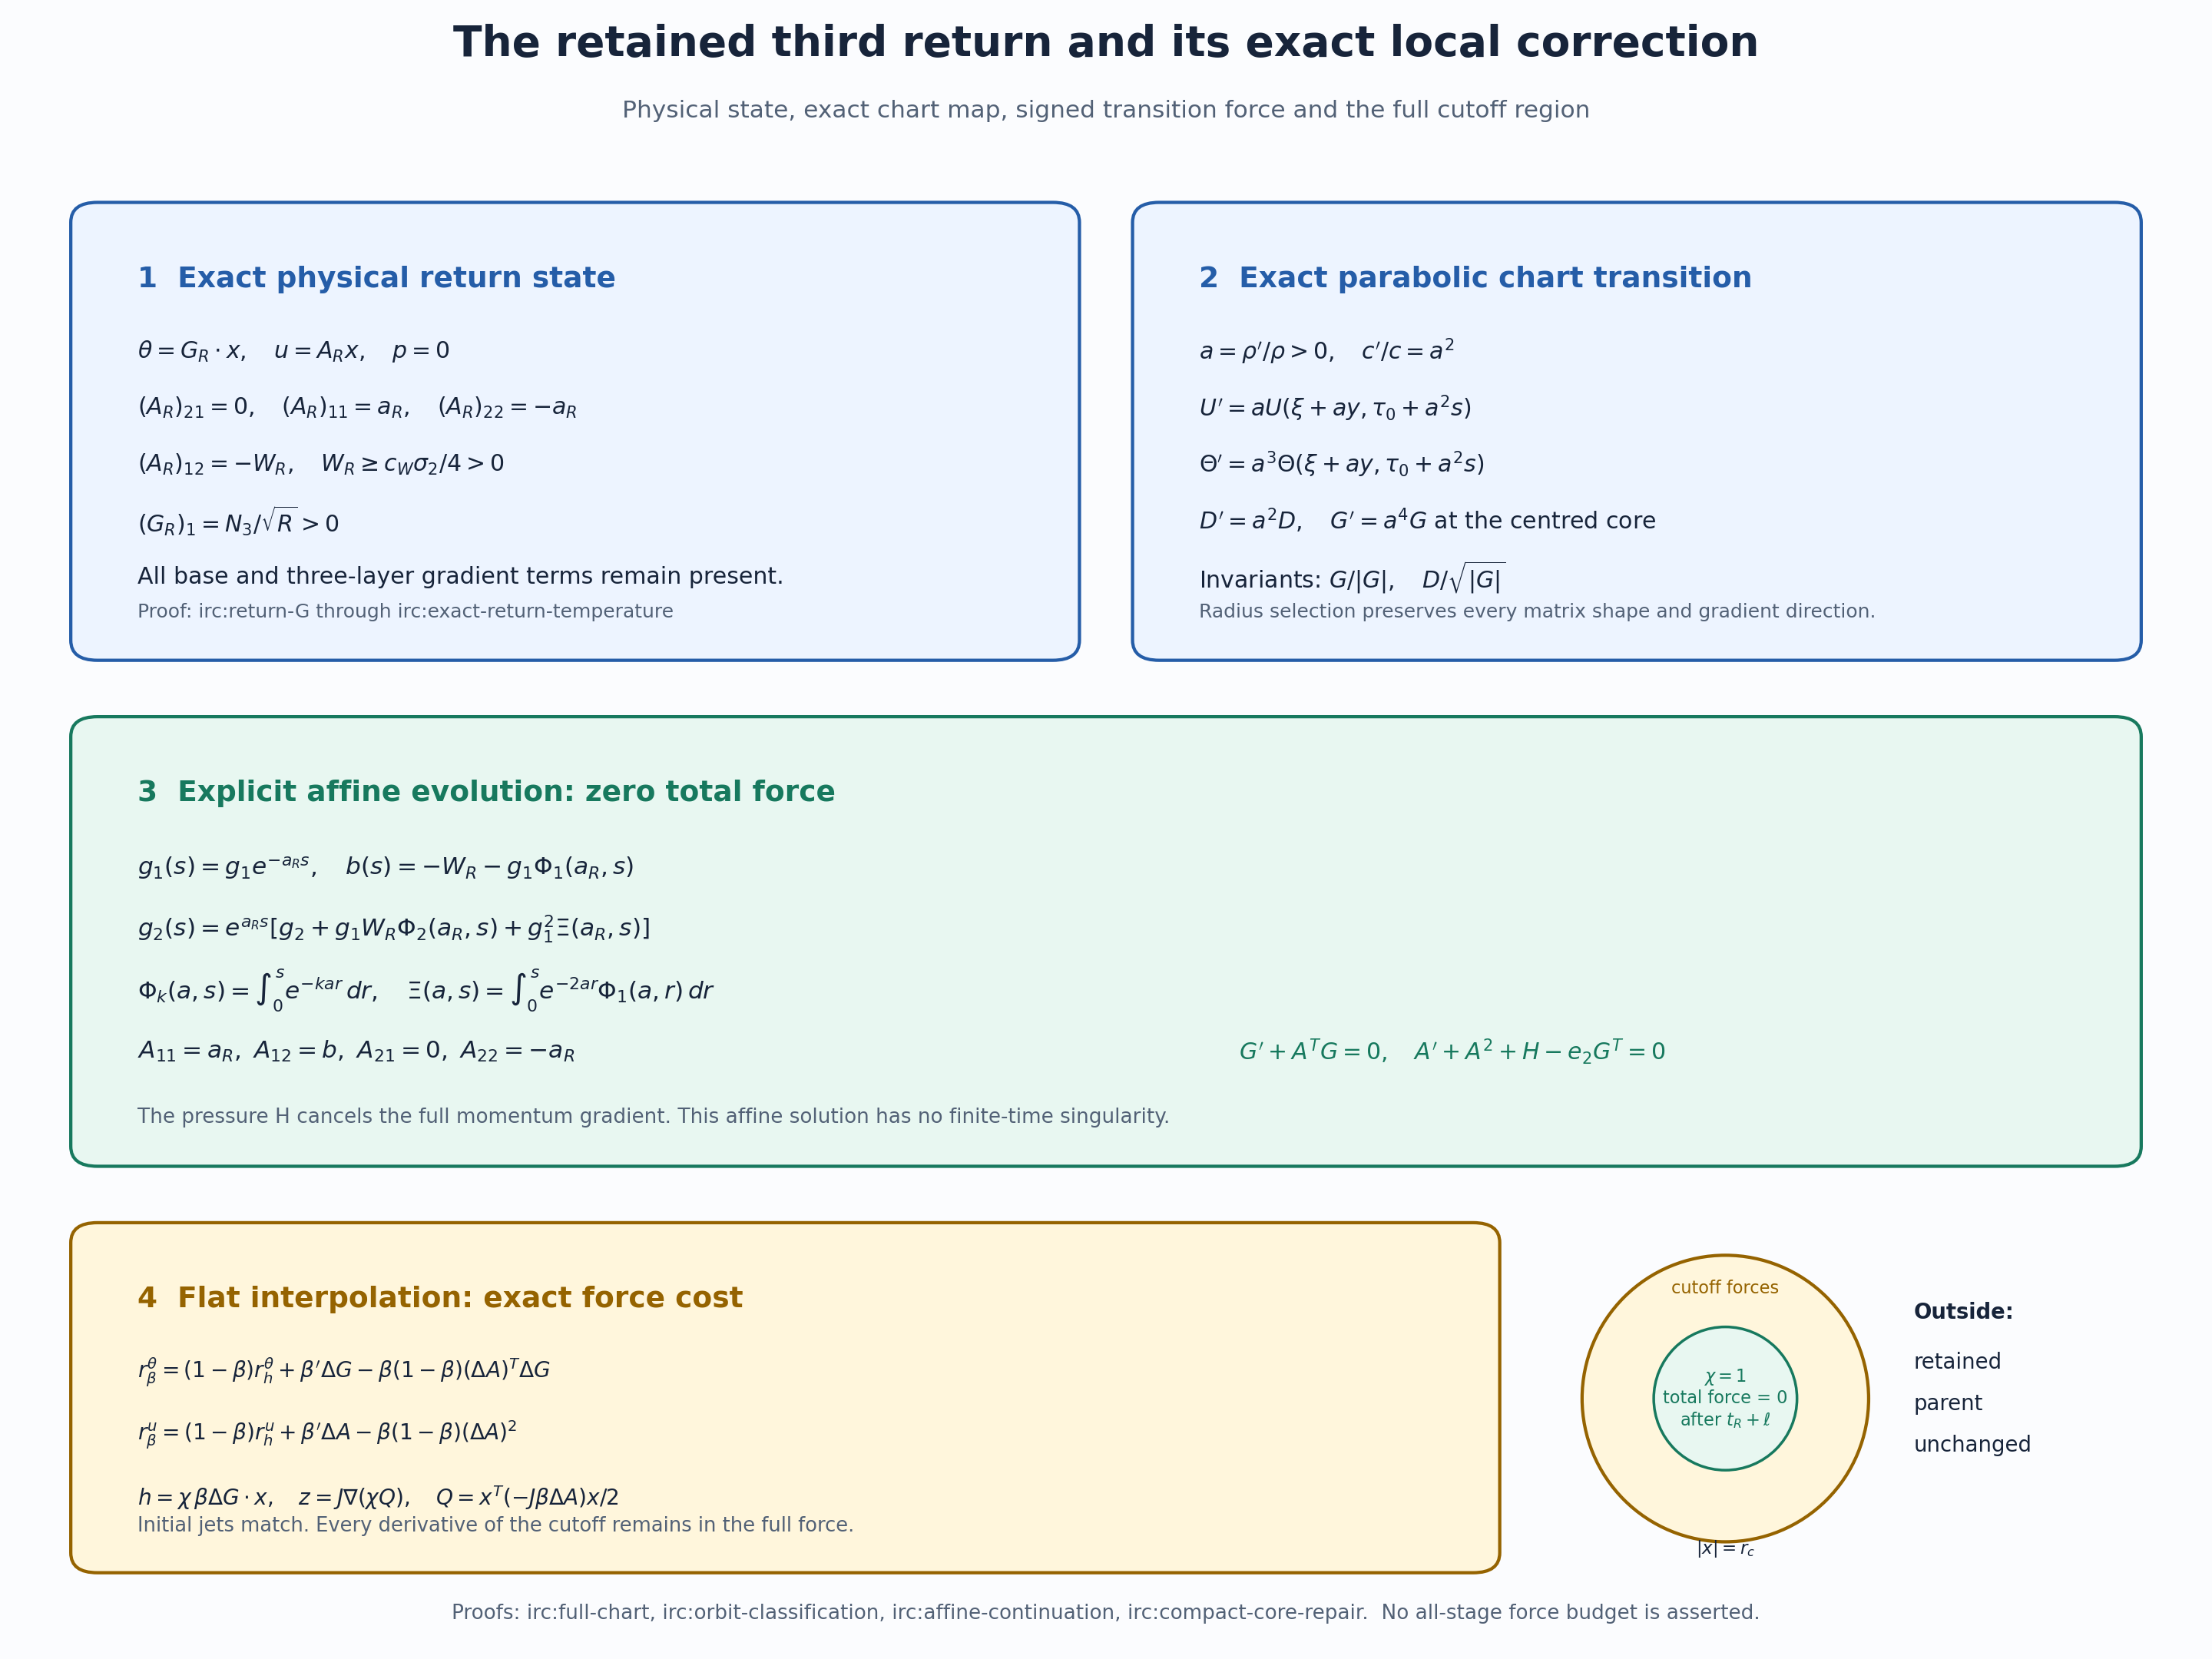
\includegraphics[width=0.97\linewidth]
 {infinite_modified/figures/return_correction.png}
 \caption{Exact third-return state and its compact local correction.
 The physical $G_1=N_3/\sqrt R$ and curl are positive, while every
 strain and vertical-gradient contribution remains present.
 Parabolic dilation preserves the displayed full state invariants.
 The explicit affine evolution cancels its total force.  A flat
 transition and a streamfunction cutoff preserve the old initial
 jets and localize the correction; their displayed signed terms
 are the force cost still to be controlled.}
 \label{irc:figure}
\end{figure}
